\clearpage
\section{Experimental implementation and rendering pipeline}
\subsection{From source geometry to a runnable model}
The experiment was built on a single Ubuntu workstation. The source CAD is the project's private \texttt{priv\_humanoid} repository at revision \texttt{171930c}. A Python assembly script loads the humanoid MJCF and repaired V3 hand model, computes a forward-facing arm pose, and replaces the original hand assemblies at the wrist joints. The two hands receive separate joint and tendon names and one pen each. Each pen has a free joint. The combined MJCF uses gravity of 9.81 m/s$^2$, the implicit-fast integrator, an elliptic friction cone, and the Newton solver with a limit of 30 iterations per 2 ms step.

\subsection{From a schedule to a trajectory}
The Python experiment runner selects a disturbance schedule by seed, constructs its time-varying loads, and advances the coupled model in MuJoCo 3.8.0. Candidate foot placements run in additional CPU processes on the same Intel Core Ultra 9 275HX. The local model copies are disposable: only the selected action is applied to the continuing physical trajectory. This preserves one continuous history for walking, finger contacts and pen motion. Wall-clock planning time is distinct from simulated time.

For each run the physics loop writes time, applied lateral force, pelvis state, foot contacts and grasp diagnostics at 500 Hz. A separate 60 Hz trace stores joint positions and named body poses for reconstruction. The evaluator uses force onsets and releases to extract event windows; it scores landings from contact and ankle position, walking from pelvis displacement, and pen reorientation from wrist and pen orientations. The complete set of seeds is reported with its failed cases in Table~\ref{tab:trials}.

\begin{center}
\sidelabel{(a) Recorded joint state in MuJoCo}\\[2pt]
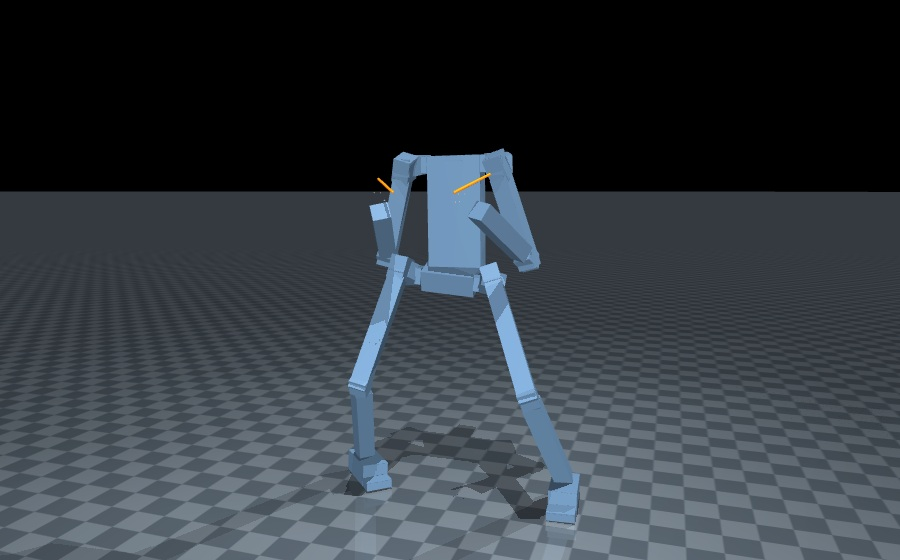
\includegraphics[width=.9\linewidth]{gorseller/physics-state.jpg}
\end{center}
\figcap{fig:physics}{The stored joint state at 18.50 s loaded back into MuJoCo. This view shows the articulated simulation geometry. Gravity, contacts and the applied load were resolved during the original rollout.}
\newpage
\subsection{From trajectory to film}
The Blender 4.5.16 production scripts bind the recorded positions and quaternions to named robot links, including the two V3 hand assemblies. The same pose samples place the pen bodies in each shot. Quaternion signs are made continuous before animation curves are written. A level studio floor, soft lights and contrasting pens aid inspection of contact and foot placement.

The full take has 3,301 pose samples including the endpoint. The first 3,300 samples drive the 55 s film at 60 frames/s. Ten cameras show the same recording in consecutive 5.5 s shots. During two push intervals, wrist-locked close-ups reuse the same frame numbers as the body view. Cycles renders the images on the workstation's NVIDIA GeForce RTX 5090 Laptop GPU with OptiX acceleration and denoising.

\begin{center}
\sidelabel{(b) Blender scene before overlays}\\[2pt]
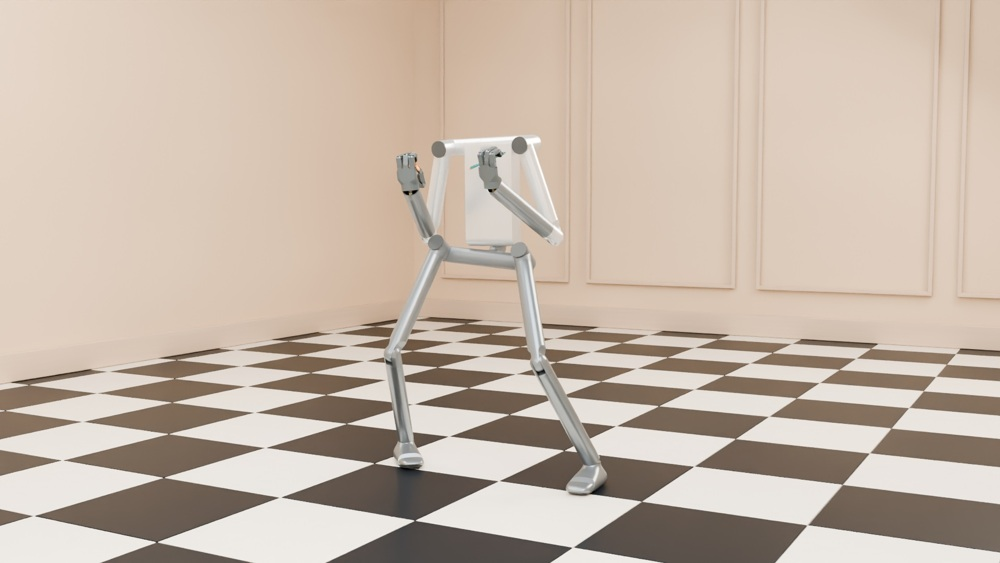
\includegraphics[width=.95\linewidth]{gorseller/blender-state.jpg}\\[4pt]
\sidelabel{(c) Decoded H.264 frame}\\[2pt]
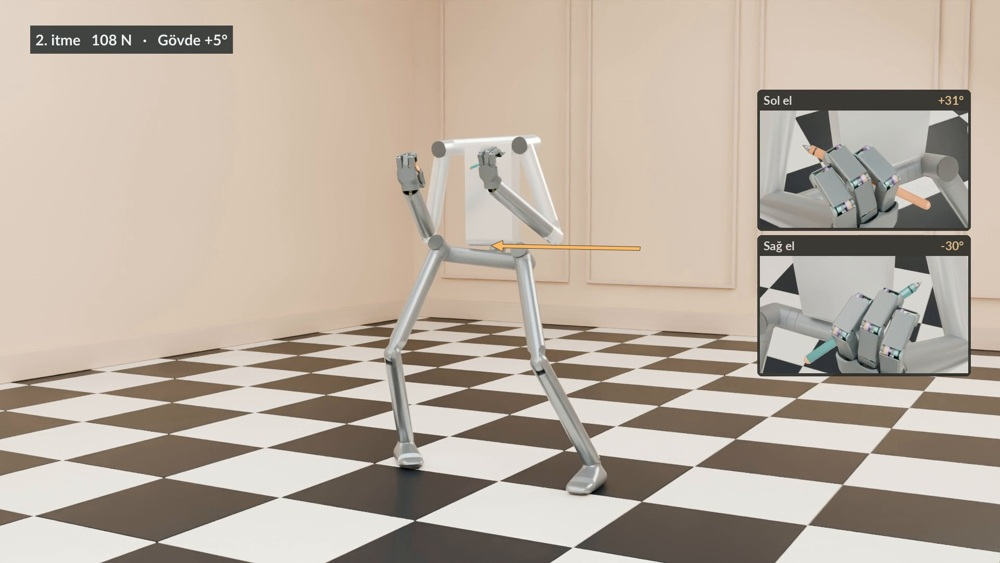
\includegraphics[width=.95\linewidth]{gorseller/encoded-frame.jpg}
\end{center}
\figcap{fig:encoding}{The same instant as Fig.~\ref{fig:physics}, before and after compositing. The encoded view adds the load direction, captions, and synchronized left and right wrist views.}
\subsection{Encoding and verification}
Python assembles the force and object-angle captions, wrist-inset overlays and chapter metadata, then invokes FFmpeg to encode H.264 at 1,920 by 1,080 pixels. The encoder uses a constant rate factor of 16. The finishing script reopens the output, checks frame count, duration, frame rate and image dimensions, and decodes frames from nine points in the film to check image content. The underlying pose and force logs remain available independently of the encoded video.
